\subsubsection{实现与数值经验}
\label{subsubsec:vms-coarse-projection-implementation}

\begin{note}[方法(8.288)的实现]
\label{note:vms-coarse-projection-implementation}
若三尺度基于投影的 VMS 方法\hyperref[eq:vms-coarse-projection-three-scale-method]{(8.288)}中的所有空间都定义在同一网格 $\mathcal T^h$ 上(见笔记\hyperref[note:vms-coarse-projection-spaces]{8.261}),则当空间 $\mathcal L^H$ 满足下列两个条件时,该方法可以高效实现:
\begin{itemize}
 \item $\mathcal L^H$ 关于网格 $\mathcal T^h$ 是不连续有限元空间;
 \item $\mathcal L^H$ 的基在 $L^2(\Omega)$ 中正交.
\end{itemize}
下面说明实现中的若干细节.记速度向量和对称张量分别为
\[
 \bm w^h=\begin{pmatrix}w_1^h\\w_2^h\\w_3^h\end{pmatrix},
 \qquad
 \bm G^H=\begin{pmatrix}
 g_{11}&g_{12}&g_{13}\\
 g_{12}&g_{22}&g_{23}\\
 g_{13}&g_{23}&g_{33}
 \end{pmatrix}.
\]
令 $\{\phi_i^h\}_{i=1}^{N_v}$ 为速度空间的标量基,令 $\{\ell_j^H\}_{j=1}^{N_L}$ 为 $\mathcal L^H$ 的标量基.空间 $V^h$ 可取基
\[
 \left\{
 \begin{pmatrix}\phi_i^h\\0\\0\end{pmatrix},
 \begin{pmatrix}0\\\phi_i^h\\0\end{pmatrix},
 \begin{pmatrix}0\\0\\\phi_i^h\end{pmatrix}
 \right\}_{i=1}^{N_v},
\]
而 $\mathcal L^H$ 可取由下列六类对称张量组成的基:
\[
\begin{gathered}
 \begin{pmatrix}\ell_j^H&0&0\\0&0&0\\0&0&0\end{pmatrix},\quad
 \frac12\begin{pmatrix}0&\ell_j^H&0\\\ell_j^H&0&0\\0&0&0\end{pmatrix},\quad
 \frac12\begin{pmatrix}0&0&\ell_j^H\\0&0&0\\\ell_j^H&0&0\end{pmatrix},\\[2mm]
 \begin{pmatrix}0&0&0\\0&\ell_j^H&0\\0&0&0\end{pmatrix},\quad
 \frac12\begin{pmatrix}0&0&0\\0&0&\ell_j^H\\0&\ell_j^H&0\end{pmatrix},\quad
 \begin{pmatrix}0&0&0\\0&0&0\\0&0&\ell_j^H\end{pmatrix},
 \qquad j=1,\ldots,N_L.
\end{gathered}
\]

对方法\hyperref[eq:vms-coarse-projection-three-scale-method]{(8.288)}作时间离散,并在当前离散时刻对对流项线性化,可得到如下线性鞍点问题:
\begin{equation}\label{eq:vms-coarse-projection-implementation-system}
\resizebox{\linewidth}{!}{$
\left(\begin{array}{cccccccccc}
 A_{11}&A_{12}&A_{13}&B_1^{\mathsf T}&\widetilde G_{11}&\widetilde G_{12}&\widetilde G_{13}&\widetilde G_{14}&\widetilde G_{15}&\widetilde G_{16}\\
 A_{21}&A_{22}&A_{23}&B_2^{\mathsf T}&\widetilde G_{21}&\widetilde G_{22}&\widetilde G_{23}&\widetilde G_{24}&\widetilde G_{25}&\widetilde G_{26}\\
 A_{31}&A_{32}&A_{33}&B_3^{\mathsf T}&\widetilde G_{31}&\widetilde G_{32}&\widetilde G_{33}&\widetilde G_{34}&\widetilde G_{35}&\widetilde G_{36}\\
 B_1&B_2&B_3&0&0&0&0&0&0&0\\
 G_{11}&G_{12}&G_{13}&0&M&0&0&0&0&0\\
 G_{21}&G_{22}&G_{23}&0&0&\frac12M&0&0&0&0\\
 G_{31}&G_{32}&G_{33}&0&0&0&\frac12M&0&0&0\\
 G_{41}&G_{42}&G_{43}&0&0&0&0&M&0&0\\
 G_{51}&G_{52}&G_{53}&0&0&0&0&0&\frac12M&0\\
 G_{61}&G_{62}&G_{63}&0&0&0&0&0&0&M
 \end{array}\right)
 \begin{pmatrix}w_1\\w_2\\w_3\\p\\g_{11}\\g_{12}\\g_{13}\\g_{22}\\g_{23}\\g_{33}\end{pmatrix}
 =
 \begin{pmatrix}f_1\\f_2\\f_3\\0\\0\\0\\0\\0\\0\\0\end{pmatrix}.
 $}
\end{equation}
若对方法\hyperref[eq:vms-coarse-projection-three-scale-method]{(8.288)}作离散时不含涉及 $\bm G^H$ 的项,也就是湍流模型作用于所有尺度,则需要组装矩阵 $A_{11},\ldots,A_{33}$ 和 $B_1,B_2,B_3$.式\hyperref[eq:vms-coarse-projection-implementation-system]{(8.323)}中的 $M$ 是 $\mathcal L^H$ 的质量矩阵,即
\[
 M_{ij}=(\ell_j^H,\ell_i^H).
\]

利用 $V^h$ 和 $\mathcal L^H$ 的上述基,可以直接计算矩阵 $G_{11},\ldots,G_{63}$ 以及 $\widetilde G_{11},\ldots,\widetilde G_{36}$ 的一般元素:
\begin{equation}\label{eq:vms-coarse-projection-implementation-blocks}
\begin{aligned}
 (G_{11})_{ij}&=(\partial_x\phi_j^h,\ell_i^H),
 &G_{22}=G_{33}&=\tfrac12G_{11},\\
 (G_{42})_{ij}&=(\partial_y\phi_j^h,\ell_i^H),
 &G_{21}=G_{53}&=\tfrac12G_{42},\\
 (G_{63})_{ij}&=(\partial_z\phi_j^h,\ell_i^H),
 &G_{31}=G_{52}&=\tfrac12G_{63},\\[1mm]
 (\widetilde G_{11})_{ij}&=(\nu_T\ell_j^H,\partial_x\phi_i^h),
 &\widetilde G_{22}=\widetilde G_{33}&=\tfrac12\widetilde G_{11},\\
 (\widetilde G_{24})_{ij}&=(\nu_T\ell_j^H,\partial_y\phi_i^h),
 &\widetilde G_{12}=\widetilde G_{35}&=\tfrac12\widetilde G_{24},\\
 (\widetilde G_{36})_{ij}&=(\nu_T\ell_j^H,\partial_z\phi_i^h),
 &\widetilde G_{13}&=\tfrac12\widetilde G_{36}.
\end{aligned}
\end{equation}
其余各块 $G_{\alpha\beta}$ 和 $\widetilde G_{\alpha\beta}$ 均为零.因此,只需组装 $G_{11},G_{42},G_{63},\widetilde G_{11},\widetilde G_{24},\widetilde G_{36}$ 这些块.若空间 $\mathcal L^H$ 不随时间变化,则 $G_{11},G_{42},G_{63}$ 和 $M$ 不含时间,可只组装一次.如果 $\nu_T$ 随时间变化,例如它依赖离散解,或者空间 $\mathcal L^H$ 随时间改变,则 $\widetilde G_{11},\widetilde G_{24},\widetilde G_{36}$ 随时间变化.

现在,可由式\hyperref[eq:vms-coarse-projection-implementation-system]{(8.323)}消去 $g_{11},\ldots,g_{33}$,从而得到关于 $(w_1,w_2,w_3,p)$ 的鞍点问题:
\begin{equation}\label{eq:vms-coarse-projection-condensed-system}
 \begin{pmatrix}
  \widetilde A_{11}&\widetilde A_{12}&\widetilde A_{13}&B_1^{\mathsf T}\\
  \widetilde A_{21}&\widetilde A_{22}&\widetilde A_{23}&B_2^{\mathsf T}\\
  \widetilde A_{31}&\widetilde A_{32}&\widetilde A_{33}&B_3^{\mathsf T}\\
  B_1&B_2&B_3&0
 \end{pmatrix}
 \begin{pmatrix}w_1\\w_2\\w_3\\p\end{pmatrix}
 =\begin{pmatrix}f_1\\f_2\\f_3\\0\end{pmatrix}.
\end{equation}
其中
\begin{align*}
 \widetilde A_{11}&=A_{11}-\widetilde G_{11}M^{-1}G_{11}
   -\tfrac12\widetilde G_{24}M^{-1}G_{42}
   -\tfrac12\widetilde G_{36}M^{-1}G_{63},\\
 \widetilde A_{12}&=A_{12}-\tfrac12\widetilde G_{24}M^{-1}G_{11},\\
 \widetilde A_{13}&=A_{13}-\tfrac12\widetilde G_{36}M^{-1}G_{11},\\[-1mm]
 &\hspace{2em}\vdots\\[-1mm]
 \widetilde A_{33}&=A_{33}-\widetilde G_{36}M^{-1}G_{63}
   -\tfrac12\widetilde G_{11}M^{-1}G_{11}
   -\tfrac12\widetilde G_{24}M^{-1}G_{42}.
\end{align*}
对 $\mathcal L^H$ 的基函数作不同的缩放,所得结果仍相同,因为缩放因子会相互抵消.

矩阵 $\widetilde G_{11}M^{-1}G_{11}$ 的第 $(i,j)$ 个元素为
\begin{equation}\label{eq:vms-coarse-projection-implementation-product}
\begin{aligned}
 (\widetilde G_{11}M^{-1}G_{11})_{ij}
 &=\sum_{m,n=1}^{N_L}(\widetilde G_{11})_{im}(M^{-1})_{mn}(G_{11})_{nj}\\
 &=\sum_{m,n=1}^{N_L}
   (\nu_T\ell_m^H,\partial_x\phi_i^h)(M^{-1})_{mn}
   (\partial_x\phi_j^h,\ell_n^H)\\
 &=\sum_{m,n=1}^{N_L}
   \left(\sum_{K\in\mathcal T^h}
      (\nu_T\ell_m^H,\partial_x\phi_i^h)_K\right)
   (M^{-1})_{mn}\\
 &\quad\cdot
   \left(\sum_{K\in\mathcal T^h}
      (\partial_x\phi_j^h,\ell_n^H)_K\right).
\end{aligned}
\end{equation}
这一公式表明,要高效实现三尺度基于投影的 VMS 方法,必须满足前述关于 $\mathcal L^H$ 的两个条件.
\begin{itemize}
 \item 若 $M$ 是对角矩阵,式\hyperref[eq:vms-coarse-projection-implementation-product]{(8.326)}便可高效计算.当且仅当 $\mathcal L^H$ 的基函数在 $L^2(\Omega)$ 中正交时,$M$ 才是对角矩阵.此时有
 \begin{equation}\label{eq:vms-coarse-projection-orthogonal-mass-product}
 \begin{aligned}
  (\widetilde G_{11}M^{-1}G_{11})_{ij}
  =\sum_{m=1}^{N_L}
  \frac{
   \displaystyle\sum_{K\in\mathcal T^h}
     (\nu_T\ell_m^H,\partial_x\phi_i^h)_K
   \,
   \displaystyle\sum_{K\in\mathcal T^h}
     (\partial_x\phi_j^h,\ell_m^H)_K}
   {\displaystyle\sum_{K\in\mathcal T^h}
     (\ell_m^H,\ell_m^H)_K}.
 \end{aligned}
 \end{equation}
 \item 高效实现还要求 $\widetilde A_{\alpha\beta}$ 的稀疏结构不比 $A_{\alpha\beta}$ 更稠密.这样,式\hyperref[eq:vms-coarse-projection-orthogonal-mass-product]{(8.327)}这类项产生的矩阵元素便可直接加到 $A_{\alpha\beta}$ 中.一般而言,只要速度基函数 $\bm v_i^h$ 与 $\bm v_j^h$ 的支集至少在一个网格单元 $K$ 上相交,元素 $(A_{\alpha\beta})_{ij}$ 就不会为零.若 $\ell_m^H$ 的支集仅覆盖一个网格单元,则式\hyperref[eq:vms-coarse-projection-orthogonal-mass-product]{(8.327)}的分子只有在该单元同时属于 $\bm v_i^h$ 和 $\bm v_j^h$ 的支集时才可能非零.此时,$\widetilde G_{11}M^{-1}G_{11}$,进而 $\widetilde A_{11}$,与 $A_{11}$ 具有相同的稀疏结构.若 $\mathcal L^H$ 是不连续有限元空间,则 $\ell_m^H$ 的支集满足这一条件.
\end{itemize}
因此,$\mathcal L^H$ 必须由分片对称张量构成,并配备 $L^2(\Omega)$ 正交基,例如 Legendre 多项式基;具有这些性质的空间见例题\hyperref[ex:appendix-b-54]{B.54}.总之,对已有不可压缩 Navier--Stokes 方程有限元程序所作的主要扩展,是依据式\hyperref[eq:vms-coarse-projection-orthogonal-mass-product]{(8.327)}这类公式组装矩阵 $\widetilde A_{ij}$,而不是 $A_{ij}$.
\end{note}

\begin{note}[投影空间 $\mathcal L^H$ 的自适应选取]
\label{note:vms-coarse-projection-adaptive-space}
自适应选取投影空间的基本想法,是将涡黏度模型集中用于流动高度湍流的子区域,并在层流子区域关闭湍流模型.
\textcite{JohnKaya2005,JohnKaya2008,JohnRoland2007,JohnKindl2010a} 对三尺度基于投影的 VMS 方法作了数值研究,采用固定空间 $\mathcal L^H=\mathbb P_0$ 和 $\mathcal L^H=\mathbb P_1^{\mathrm{disc}}$.\textcite{JohnKindl2010a} 的结论是:投影空间的选取对结果的影响远大于涡黏度模型的选取;例题\hyperref[ex:vms-coarse-projection-channel-flow]{8.277}也可参见这一比较.

\textcite{JohnKindl2010b} 提出了投影空间自适应选取的三尺度基于投影 VMS 方法.模拟过程中,投影空间可以改变,既可以每个时间步都改变,也可以隔较长时间间隔改变.在湍流强烈的子区域,局部投影空间取较小;湍流强度越弱,投影空间就取得越大.局部湍流强度由局部小的已解析尺度的大小估计:
\begin{equation}\label{eq:vms-coarse-projection-local-turbulence-intensity}
 \zeta_K=
 \frac{\|\bm G^H-D(\bm w^h)\|_{L^2(K)}}
      {\|1\|_{L^2(K)}}
 =\frac{\|\bm G^H-D(\bm w^h)\|_{L^2(K)}}{|K|^{1/2}},
 \qquad\forall K\in\mathcal T^h.
\end{equation}
随后按以下规则为每个单元选取局部投影空间.给定三个非负常数 $C_1\le C_2\le C_3$,以及一个参考值 $\zeta$(例如 $\{\zeta_K\}_{K\in\mathcal T^h}$ 关于空间或时空的某种平均值),对每个 $K$ 取:
\begin{itemize}
 \item 若 $\zeta_K/\zeta\le C_1$,取 $\mathcal L^H(K)=\mathbb P_2^{\mathrm{disc}}(K)$、$\nu_T(K)=0$,即关闭该处的湍流模型;
 \item 若 $C_1<\zeta_K/\zeta\le C_2$,取 $\mathcal L^H(K)=\mathbb P_1(K)$;
 \item 若 $C_2<\zeta_K/\zeta\le C_3$,取 $\mathcal L^H(K)=\mathbb P_0(K)$;
 \item 若 $C_3<\zeta_K/\zeta$,取 $\mathcal L^H(K)=\{0\}$,即在单元 $K$ 上,湍流模型作用于所有已解析尺度.
\end{itemize}
由于 $\mathcal L^H$ 是不连续有限元空间,在不同网格单元上指定不同的局部空间并无困难.

\textcite{JohnKindl2010b} 的数值研究表明,采用估计量\hyperref[eq:vms-coarse-projection-local-turbulence-intensity]{(8.328)}时,空间 $\mathcal L^H$ 的分布确实符合预期.对 $\mathrm{Re}_\tau=180$ 的湍流槽道流(见例题\hyperref[ex:appendix-d-12]{D.12}),壁面处取 $\mathcal L^H(K)=\{0\}$,而槽道中央关闭湍流模型.对绕圆柱的湍流流动(见例题\hyperref[ex:appendix-d-13]{D.13}),圆柱附近取 $\mathcal L^H(K)=\{0\}$;远离圆柱且不处于尾流中的区域则关闭湍流模型,见图\hyperref[fig:vms-adaptive-cylinder-flow]{8.17}.这些研究采用六面体网格及 $Q_2/\mathbb P_1^{\mathrm{disc}}$ 空间对,见笔记\hyperref[note:qk-pdisc-mapped-unmapped]{3.141}.\textcite{JohnKindlSuciu2010} 将自适应基于投影的 VMS 方法推广到四面体网格,采用 Bernardi--Raugel 元 $P_2^{\mathrm{BR}}/\mathbb P_1^{\mathrm{disc}}$,见笔记\hyperref[note:bernardi-raugel-second-order-3d]{3.140}.
\end{note}

\begin{example}[($\mathrm{Re}_\tau=180$ 的湍流槽道流)]
\label{ex:vms-coarse-projection-channel-flow}
本例的定义见例题\hyperref[ex:appendix-d-12]{D.12},模拟设置与例题\hyperref[ex:smagorinsky-turbulent-channel]{8.128}中所述完全相同.

\begin{elegantfigure}[1.055\linewidth]
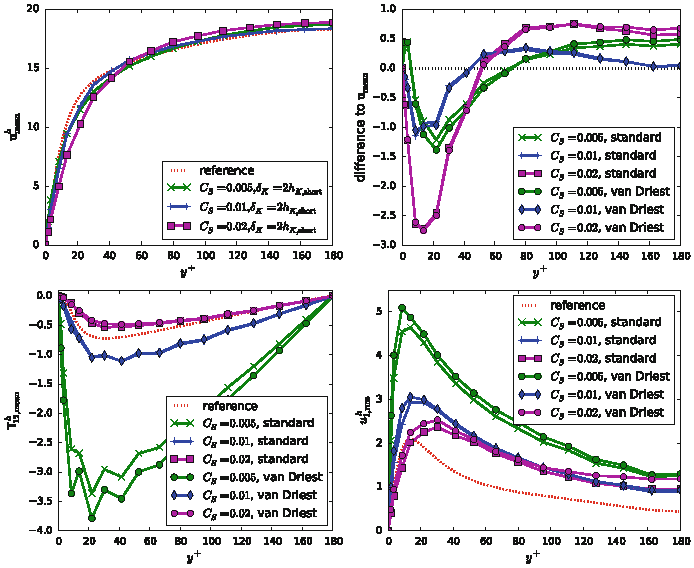
\includegraphics[width=\linewidth]{figures/Chapter_08/Fig_8_11__PDFp648__Bookp639.pdf}
\captionof{figure}{例题\hyperref[ex:vms-coarse-projection-channel-flow]{8.277}:采用 $\mathcal L^H=\mathbb P_0$ 的三尺度粗空间投影 VMS 方法\hyperref[eq:vms-coarse-projection-three-scale-method]{(8.288)}所得的若干统计量.}
\label{fig:vms-channel-p0-statistics}
\end{elegantfigure}

图\hyperref[fig:vms-channel-p0-statistics]{8.11}、\hyperref[fig:vms-channel-p1-statistics]{8.12}和\hyperref[fig:vms-channel-adaptive-statistics]{8.13}分别给出了 $\mathcal L^H=\mathbb P_0$、$\mathcal L^H=\mathbb P_1^{\mathrm{disc}}$ 以及自适应选取投影空间时,三尺度粗空间投影 VMS 方法\hyperref[eq:vms-coarse-projection-three-scale-method]{(8.288)}的结果.

正如笔记\hyperref[note:vms-dynamic-smagorinsky-common-goal]{8.216}所述,三尺度 VMS 方法的目标之一,是限制 Smagorinsky 模型直接作用于小的已解析尺度,从而降低该模型的影响.结果表明,这一目标确已实现:与 Smagorinsky 大涡模拟模型相比,该方法在更宽的 $C_S$ 参数范围内都能给出合理结果,见图\hyperref[fig:smagorinsky-channel-flow]{8.4}.VMS 方法在较大的 $C_S$ 取值下结果最准确.与 Smagorinsky 大涡模拟模型类似,采用 van Driest 阻尼\hyperref[eq:van-driest-damping]{(8.152)}的影响很小.标准 Smagorinsky 方法的结果往往略为准确,但并非总是如此.

\begin{elegantfigure}[1.055\linewidth]
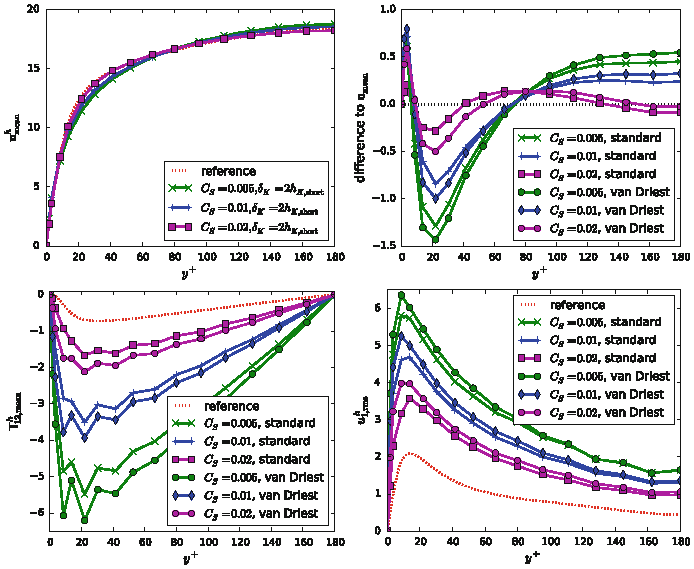
\includegraphics[width=\linewidth]{figures/Chapter_08/Fig_8_12__PDFp649__Bookp640.pdf}
\captionof{figure}{例题\hyperref[ex:vms-coarse-projection-channel-flow]{8.277}:采用 $\mathcal L^H=\mathbb P_1^{\mathrm{disc}}$ 的三尺度粗空间投影 VMS 方法\hyperref[eq:vms-coarse-projection-three-scale-method]{(8.288)}所得的若干统计量.}
\label{fig:vms-channel-p1-statistics}
\end{elegantfigure}

\begin{elegantfigure}[1.055\linewidth]
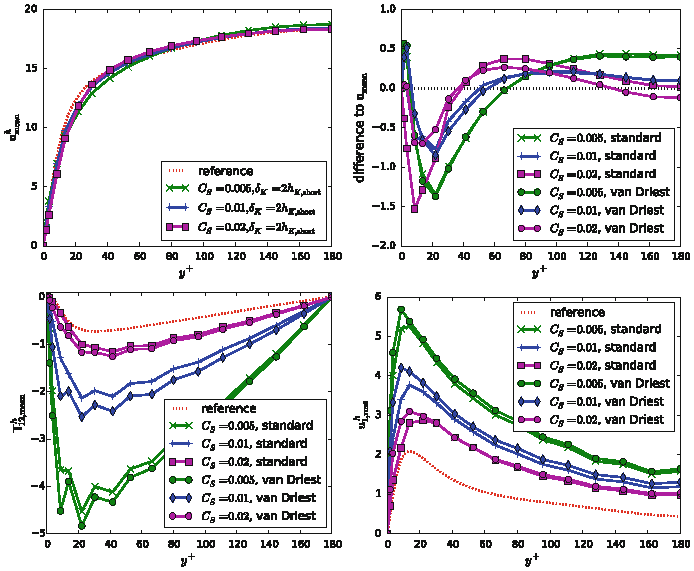
\includegraphics[width=\linewidth]{figures/Chapter_08/Fig_8_13__PDFp650__Bookp641.pdf}
\captionof{figure}{例题\hyperref[ex:vms-coarse-projection-channel-flow]{8.277}:自适应选取投影空间时,三尺度粗空间投影 VMS 方法\hyperref[eq:vms-coarse-projection-three-scale-method]{(8.288)}所得的若干统计量.}
\label{fig:vms-channel-adaptive-statistics}
\end{elegantfigure}
\end{example}
\index{变分多尺度方法!基于粗空间投影!实现}
\index{变分多尺度方法!基于粗空间投影!自适应投影空间}
\index{投影空间!自适应选取}


